\documentclass{beamer}
\usepackage{listings}
\lstset{
%language=C,
frame=single, 
breaklines=true,
columns=fullflexible
}
\usepackage{graphicx}
\usepackage{subcaption}
\usepackage{url}
\usepackage{tikz}
\usepackage{tkz-euclide}
\usetikzlibrary{calc,math}
\usepackage{float}
\newcommand\norm[1]{\left\lVert#1\right\rVert}
\renewcommand{\vec}[1]{\mathbf{#1}}
\usepackage[export]{adjustbox}
\usepackage[utf8]{inputenc}
\usepackage{amsmath}
\usetheme{Boadilla}
\title{Optimisation of SFD  in HD LoRa Networks}
\author{S. Rithvik Reddy}
\institute{IIT H (CSE)}
\date{\today}
\begin{document}

\begin{frame}
\titlepage
\end{frame}

\begin{frame}
\frametitle{What is HD LoRa networks ?}

$\bullet$ It stands for High Density Long Range networks.\\
$\bullet$ LoRa wireless technology has the capability for long range, low bit rate, low power communiocations which, makes it an ideal solution in many Smart City and Industrial Internet of Things (IOT).\\
$\bullet$ LoRa uses Chirp Spread Spectrum (CSS) technology.\\
$\bullet$ CSS is a spread spectrum technique that uses wideband linear frequency modulated chirp pulses to encode information.\\
$\bullet$ A chirp is a sinusoidal signal whose frequency denpends on time in a polynomial fashion. 

\end{frame}


\begin{frame}
\frametitle{What is SFD ?}

$\bullet$ SFD stands for Spreading Factor Distribution.\\
$\bullet$ The number of chirps required to carry a bit is known as spreading factor.\\
$\bullet$ CSS uses spreading factors from 7 to 12. The higher the SF higher the time taken for transmission.
\begin{block}{Distribution}
$\bullet$ In smart cities there will be a large no of appliances using LoRa networks and each transmit their own data.\\
$\bullet$ If proper care is not taken due to the high density of nodes, packet collisions may occur and data will be lost.\\
$\bullet$ one way to avoid this is to use proper SF for individual node to avoid collisions as best as we can.
\end{block}

\end{frame}


\begin{frame}
\frametitle{Packet collision}

$\bullet$ LoRaWAN- Long range wide area network.\\
$\bullet$ Imagine a big Amazon pantry store house and distributing facility where LoRa is used to  transmitting temperature, humidity, vibration, lighting and similar data of various parts of storage units from some smart appliances.\\
$\bullet$ Now each appliance will act as a node transmitting it's own data.\\
\begin{figure}[h]
    \centering
    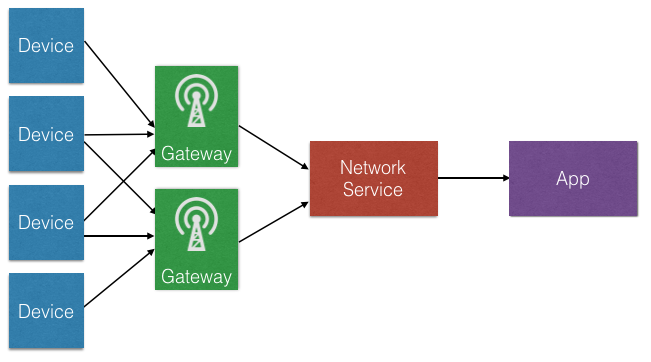
\includegraphics[width=0.4\textwidth]{img-1}
\end{figure}
$\bullet$ LoRaWAN uses pure \textbf{ALOHA} transmission protocol.\\ 
$\bullet$ ALOHA is a system for coordinating and arbitrating access to a shared communication Networks channel.\\

\end{frame}


\begin{frame}
\frametitle{Pure ALOHA}
$\bullet$ In pure ALOHA, the stations transmit frames whenever they have data to send. That means the nodes won't listen before transmitting data.\\
$\bullet$ So if the gateway is busy and node transmits a message at same frequency then a collision may occur which leads to loss of data.\\
$\bullet$ In pure ALOHA, whenever any station transmits a frame, it expects the acknowledgement from the receiver.\\
$\bullet$ If acknowledgement is not received within specified time, the station assumes that the frame has been destroyed.\\
$\bullet$ Now the station waits for a random amount of time and sends it again this time with higher SF.\\
$\bullet$ This will further worsen the situation as the SF increases time of transmission will increase and it will increase the probability of collision.\\
$\bullet$ Now imagine the situation of smart cities where Gateway traffic (or node density) is very high. 

\end{frame}


\begin{frame}
\frametitle{Optimising LoRaWAN}
$\bullet$ while in case of a small case use like in a small store house this may not be a problem but consider cases like an appliance sending traffic updates or water supply routes and duration in a big city.
\begin{block}{Factors}
\begin{enumerate}
\item Spreading Factor (SF)
\item Transmission Power (TP)
\item Band Width (BW)
\item Coding Rate (CR)
\item Pay Load (PL)
\end{enumerate}
\end{block}

\end{frame}


\begin{frame}
\frametitle{A Possible solution}
 
 One way to work around this problem is to make sure that while one node is transmitting other node transmitting at the same frequency should not transmit the message.\\
$\blacktriangleright$ But this can't be done by nodes as they wont listen before transmitting the message.\\
$\blacktriangleright$ To get around this problem we can distribute SF among the nodes in such a way such that the probability of collision will be as low as possible.\\
$\blacktriangleright$ This boils down to the case of optimising SFD in such away such that no collision will occur while message is being transmitted.\\ 

\end{frame}


\begin{frame}
\frametitle{Time taken for transmission of a message}
\begin{align}
&T_{sym}=\dfrac{2^{SF}}{BW}
\end{align}
BW- Band width\\
$\bullet$ let $T_{pkt}$ be time needed to transmit a data packet via the LoRa radio interface, in this we should also consider LoRa modulation details.
\begin{figure}[h]
    \centering
    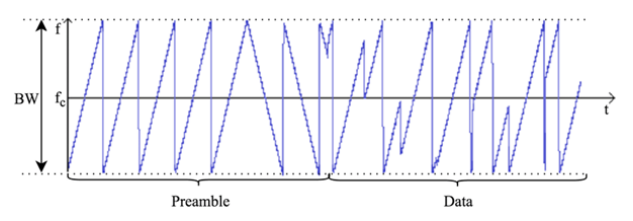
\includegraphics[width=0.5\textwidth]{img-2}
    \caption{LoRa Packet Form}
\end{figure}
so
\begin{align}
T_{pkt}=T_{pre}+T_{phy}
\end{align}

\end{frame}


\begin{frame}
\frametitle{Time taken for transmission of a message}
\begin{align}
&T_{pre}=(N_{pre}+4.25)T_{sym}\\
\implies&T_{pre}=(N_{pre}+4.25)\left(\dfrac{2^{SF}}{BW}\right)
\end{align}
Let us define a variable TEMP as
\begin{align}
TEMP=\dfrac{(28+8PL+16CRC-4SF-20IH)}{4(SF-2DE)}
\end{align}
TERMS:\\
PL - payload size(bytes)\\
CRC- cyclic redundancy check(error detecting code)\\
IH - Implicit Header(IH=1 if used else 0)\\
DE - 1 if data rate optimisation is used 0 otherwise\\ 
CR - code rate (lies between 1 and 4)

\end{frame}


\begin{frame}
\frametitle{Time taken for transmission of a message}
Then the total Physical layer payload size $N_{pl}$ is given by
\begin{align}
&Npl = 8 + max[ceil[TEMP](CR+4),0]\\
\implies & T_{phy}=  (8 + max[ceil[TEMP](CR+4),0]\left(\dfrac{2^{SF}}{BW}\right)
\end{align}
Hence the total Lora packet transmission time, $T_{pkt}$, is given by,
\begin{align}
T_{pkt} =(N_{pre} + 4.25 + (8 + max[ceil[TEMP](CR+4),0]))\left(\dfrac{2^{SF}}{BW}\right)
\end{align}

\end{frame}


\begin{frame}
\frametitle{Frame Success Probability Analysis}
Packet collision in a LoRa network can be divided into two types: Intra-SF collisions and Inter-SF collisions.\\
Consider a Node - Gateway system as shown.
\begin{figure}[h]
    \centering
    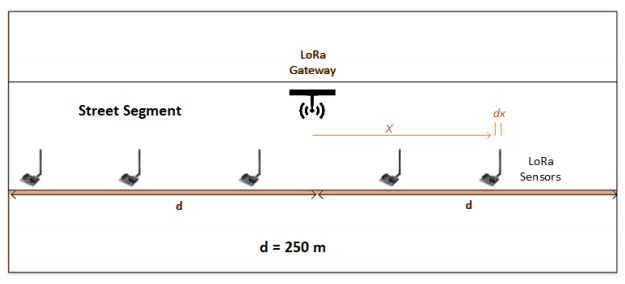
\includegraphics[width=0.5\textwidth]{img-3}
    \caption{Typical Smart City Street Segment with one Gateway}
\end{figure}
\begin{block}{Intra-SF collisions}
$\bullet$ Collision occurs between two LoRa frames with the same frequency and SF. In this case, only the LoRa frame with the highest power can be decoded. This happens when its power at the gateway is at least 6 dB more than the other one.

\end{block}

\end{frame}


\begin{frame}
\frametitle {Intra-SF collisions}
$\bullet$ Now, let us consider a node, transmitting a packet at distance x from the gateway.\\
$\bullet$ Considering fixed conditions and all nodes (N) have the same transmission parameters, the received power level only depends on the distance. Hence, the potential intra-SF interferes are those whose distance from the gateway is below xR with
\begin{align}
R=e^{\frac{6}{10\gamma}}
\end{align}
where, $\gamma$ is path-loss coefficient.\\
let $\alpha_i,i\in [7,12]$ denotes the fraction of nodes with SF=i.
\begin{align}
\implies \sum_{i=7}^{12} \alpha_i
=1\end{align}
And if $D_i$ denotes the density of nodes having SF equal to $SF_i$ then 
\begin{align}
D_i=\dfrac{\alpha_iN}{2d}
\end{align}
 
\end{frame}


\begin{frame}
\frametitle{Inter-SF collisions}
\begin{block}{Inter-SF collisions}
$\bullet$ Collision occurs between two LoRa frames with the same frequency and different SF.\\
$\bullet$ In this case, the first frame is demodulated only if the difference between the received power of the first frame and the second frame is higher than the Signal-to-Interference Ratio (SIR) of the first one. 

\end{block}
\begin{table}[h!]
  \begin{center}
    \caption{MINIMUM SIR REQUIRED TO DEMODULATE $SF_i$}
    \begin{tabular}{|l|c|c|c|c|c|r|}
    \hline 
     SIR Margin (dB) & SF7 & SF8 & SF9 & SF10 & SF11 & SF12\\
      \hline
      SF7 &  & -8 & -9 & -9 & -9 & -9\\
      \hline
      SF8 & -11 &  & -11 & -12 & -13 & -13\\
      \hline
      SF9 & -15 & -13 &  & -13 & -14 & -15\\
      \hline
      SF10 & -19 & -18 & -17 &  & -17 & -18\\
      \hline
      SF11 & -22 & -22 & -21 & -20 &  & -20\\
      \hline
      SF12 & -25 & -25 & -25 & -24 & -23 & \\
      \hline
    \end{tabular}
  \end{center}
\end{table}

\end{frame}


\begin{frame}
\frametitle{Inter-SF collisions}
$\bullet$ Now consider the same case of a node, transmitting a packet at distance x from the gateway with $SF_i$ spreading factor.\\
$\bullet$ The potential inter-SF interferers are those whose distance from the gateway is below xQ. Where,
\begin{align}
Q= e^{\dfrac{SIR[i,j]}{10\gamma}}
\end{align}
Where $SF_j$ is the spreading factor of colliding packet.\\
Also D represents density of nodes is given by $D=\dfrac{N}{2d}$.
\end{frame}

\begin{frame}
\frametitle{Probability of a successful transmission}
\begin{align}
\text{Total Interferers} = D_i.R.x + D.Q.x
\end{align}
Assuming that the data transmissions follow a Poisson distribution with rate $2dD \theta$ where, $\theta$ is packet transmission intensity (packets per second).
$\bullet$  The probability of observing k events in an interval is given by,
\begin{align}
P[k]=e^{\lambda} \dfrac{\lambda^k}{k!}
\end{align}
Probability of successful transmission $P_{success}(x)$ is therefore the probability that within a vulnerable period of duration $2T_{pkt}$, none of those potential interfering nodes started a transmission. Hence, the success probability is given by:
\begin{align}
P_{success}(x) \approx e^{-2T_{pkt} \theta (D_iRx+DQx)}
\end{align}

\end{frame}


\begin{frame}
\frametitle{Probability of a successful transmission}
Therefore, the average success probability for a specific SF among all nodes in the 2d length system is given by the following equation,
\begin{align}
& P_{average}^i \approx \dfrac{1}{D_i d} \int_{x=0}^{d} D_i e^{-2T_{pkt} \theta (D_iRx+DQx)}\,dx\\
\implies & P_{average}^i \approx \left(\dfrac{1}{d}\right) \left(\dfrac{1-e^{-2T_{pkt} \theta (D_iRd+DQd)}}{2T_{pkt} \theta (D_i R+DQ)}\right),i \in [7,12]
\end{align}
\end{frame}


\begin{frame}
\frametitle{Optimising probability}
$\blacktriangleright$ Having the probability of success for each SF value we now have to distribute different SF values to different nodes in our channel to get max probability of success.
\begin{enumerate}
\item Objective function \\
$P_{average}^i \approx \left(\dfrac{1}{d}\right) \left(\dfrac{1-e^{-2T_{pkt} \theta (D_iRd+DQd)}}{2T_{pkt} \theta (D_i R+DQ)}\right)$\\
\item Variables : $SF_i, T_{pkt}, \alpha_i, D_i, Q$\\
\item Constraints
\begin{align}
& 0\leq \alpha_i\leq1\\
& \alpha_7+\alpha_8+\alpha_9+\alpha_{10}+\alpha_{11}+\alpha_{12}=1
\end{align}
\end{enumerate}
Using the algorithms like golden section search and parabolic interpolation distribution of SF for max value of the probability can be found.

\end{frame}


\begin{frame}
\frametitle{A demonstration}
The above probability model was evaluated using the parameters in table below. It was assumed that all the nodes are
located within 250 m from a single gateway and SFs are equally distributed among the nodes.
\begin{table}[h!]
  \begin{center}
    \begin{tabular}{|l|r|}
    \hline 
    Parameters & value\\
    \hline
    \hline
    Number of nodes (N) & 1200\\
    \hline
    Node Transmission Interval & 10 min\\
    \hline
	Code Rate (CR) & 4/5\\
	\hline
	Bandwidth (BW) & 125KHz\\
	\hline
	Spreading Factor (SF) & 7-12\\
	\hline
	Payload(PL) & 40bytes\\
	\hline
	Low data rate optimization (DE) & 1\\
	\hline
	Header(H) & 0\\
	\hline
	Preamble symbols(np) & 8\\
	\hline
	Transmission power ($P_{tx}$) & 14 dBm\\
	\hline
	Path loss exponent ($\gamma$) & 4\\
	\hline

      
    \end{tabular}
  \end{center}
\end{table}

\end{frame}


\begin{frame}
\frametitle{With out optimisation}
$\bullet$ Success probabilities were first evaluated without any optimization. Based on the results, average probability of success
is \textbf{58.1\%} if no of nodes with each spreading factor is same.
\begin{figure}[h]
    \centering
    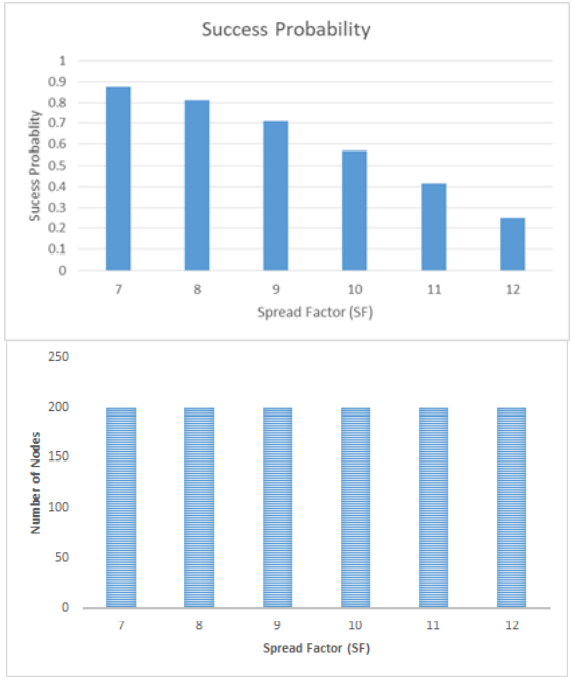
\includegraphics[width=0.45\textwidth]{img-4}
\end{figure}

\end{frame}

\begin{frame}
\frametitle{With optimisation}
$\bullet$ Based on the optimization results, average probability of success is 82.0\%. This results indicate that LoRa capacity can be increased significantly by assigning appropriate SF to the nodes.
\begin{figure}[h]
    \centering
    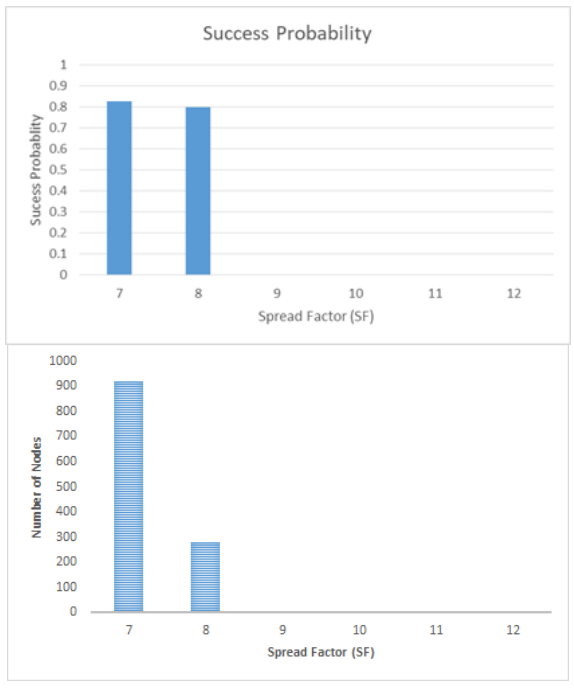
\includegraphics[width=0.45\textwidth]{img-5}
\end{figure}

\end{frame}


\end{document}